\documentclass[12pt]{article}
\usepackage[paper=letterpaper,margin=2cm]{geometry}
\usepackage{amsmath}
\usepackage{amssymb}
\usepackage{amsfonts}
\usepackage{newtxtext, newtxmath}
\usepackage{enumitem}
\usepackage{titling}
\usepackage[colorlinks=true]{hyperref}
\usepackage{graphicx}
\usepackage{csvsimple}
\usepackage{luacode}
\documentclass{article}

\usepackage{algorithm}
\usepackage{algpseudocode}
\setlength{\droptitle}{-6em}

% Enter the specific assignment number and topic of that assignment below, and replace "Your Name" with your actual name.

\title{\textbf{COMP0078 Assignment 2}}
\author{Student Numbers: 21168615 \& 19004608 \\ }
\date{Dec 14, 2022}

\begin{document}
    \maketitle
\section{PART I}
\subsection{Kernel Perceptron}
\subsubsection{Experimental Results}

\begin{itemize}
    \item[1.] To generalise the kernel perceptron to $K$ classes:
    \begin{algorithm}
    \caption{An training algorithm for multi-class kernel perceptron}\label{alg:cap}
    \begin{algorithmic}
    \For{$k\in\{1, 2, ..., K\}}$ \Comment Initialise weights for first training example

    \EndFor

    \For{$i\in\{1, 2, ..., M\}$}: \Comment Number of Epochs
        \For{$j\in\{2, ..., N\}}$ \Comment Number of training points
            \For{$k\in\{1, 2, ..., K\}}$ \Comment Number of classes
                \State $\hat{y}_k^{i, j} \gets  \sum_{i'=1}^{i-1} \sum_{j'=1}^{j-1} ( w^{i, j}_k \cdot  k(\textbf{x}_{j'}, \textbf{x}_j)} )$ \Comment{Prediction for class $k$ with kernel $k(\cdot, \cdot)$}
                \If{$sign(\hat{y}_k^{i, j}) \neq sign(y_k^{i, j})$} \Comment Compare predicted $\hat{y}_k^{i, j}$ and actual $y_k^{i, j})$
                    \State $w^{i, j}_{k} \gets y_k^{i, j}$
                \Else
                    \State $w^{i, j}_{k} \gets 0$
                \EndIf
            \EndFor
        \EndFor
    \EndFor
    \end{algorithmic}
    \end{algorithm}

    The number of epochs was determined by training on the mini train data set until the performance of the mini test set no longer changed.
    This was considered a reasonable number of epochs to use to train the actual data set.

    For prediction, the $k$ with the maximum value of $\hat{y}_k$ (the argmax of $\hat{y}$) is considered the class prediction by the model.
    \newpage

    Basic Results:

    \begin{figure}[h]
    \centering
    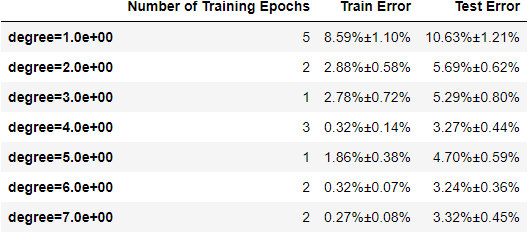
\includegraphics[scale=0.5]{outputs/part1/q1.png}
    \caption{20 Runs with a Polynomial Kernel}
    \label{fig:1}
    \end{figure}

    \item[2.] Cross Validation Results:

    \begin{figure}[h]
    \centering
    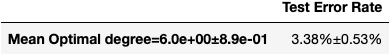
\includegraphics[scale=0.5]{outputs/part1/q2.png}
    \caption{5-fold Cross-Validation for 20 Runs with a Polynomial Kernel}
    \label{fig:2}
    \end{figure}
\newpage

    \item[3.] Confusion Matrix:

    \begin{figure}[h]
    \centering
    \begin{minipage}{.5\textwidth}
      \centering
      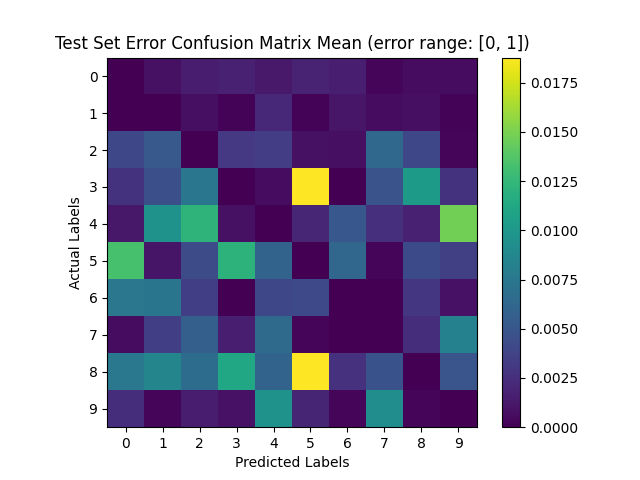
\includegraphics[width=.8\linewidth]{outputs/part1/q3_confusion-imshow_mean.png}
      \caption{Polynomial Kernel Mean}
      \label{fig:3}
    \end{minipage}%
    \begin{minipage}{.5\textwidth}
      \centering
      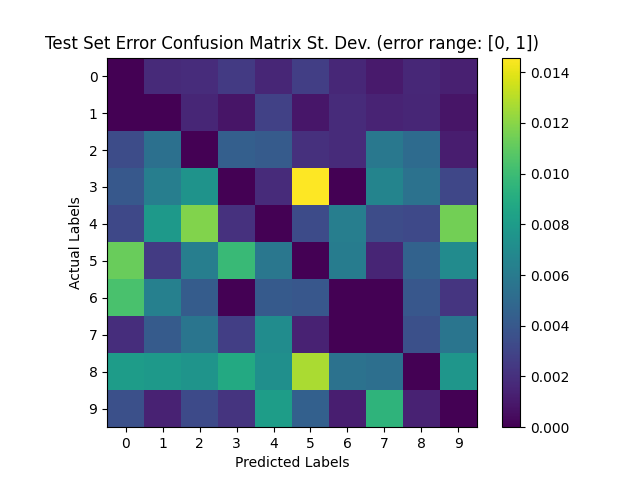
\includegraphics[width=.8\linewidth]{outputs/part1/q3_confusion-imshow_stdev.png}
      \caption{Polynomial Kernel St. Dev.}
      \label{fig:4}
    \end{minipage}
    \end{figure}

    \begin{figure}[h]
    \centering
    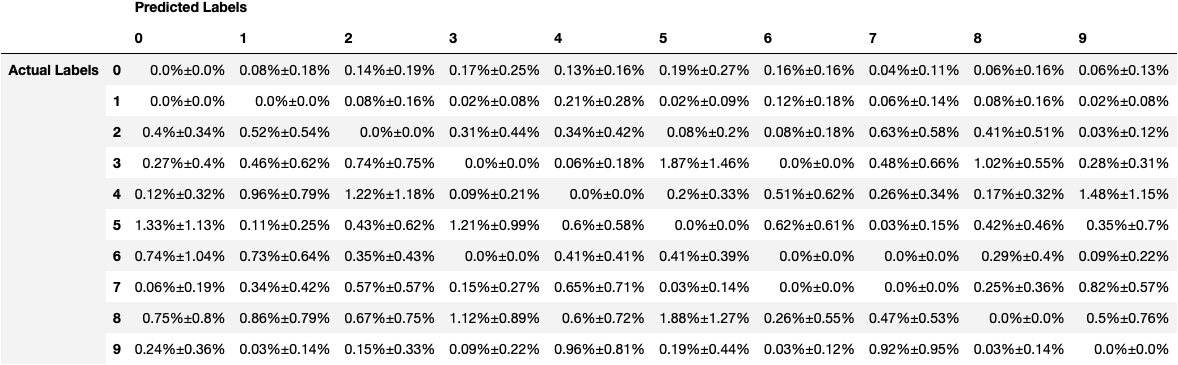
\includegraphics[scale=0.5]{outputs/part1/q3_confusion.png}
    \caption{Polynomial Kernel Confusion Matrix Error Rate Table}
    \label{fig:5}
    \end{figure}


    \item[4.] The images with the most errors made by the 20 models trained with cross-validation were considered the hardest to predict and visualised.
    It is not surprising that these are to predict. 
    We can see that in all five cases in Figure~\ref{fig:6}, the images do not look like their labels, in fact, they mostly look vertical or horizontal bars.
    Thus it would be unreasonable to expect that the model would be able to predict them correctly.

    \begin{figure}[h]
    \centering
    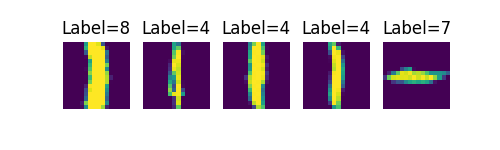
\includegraphics[scale=0.7]{outputs/part1/q4.png}
    \caption{Images with the Most Errors from the Trained Models}
    \label{fig:6}
    \end{figure}

    \newpage

    \item[5.] To select a good range of values for kernel width sigma for the Gaussian kernel, the mini training and test set was used to quickly gauge the test error for different hyper-parameters.
    The hyper-parameter values above and below the best performing hyper-parameter (with respect to test set error) was chosen as the hyper-parameter range to define $S$, the set of values for cross-validation for repeating parts 1 and 2 with the Gaussian Kernel.
    \begin{figure}[h]
    \centering
    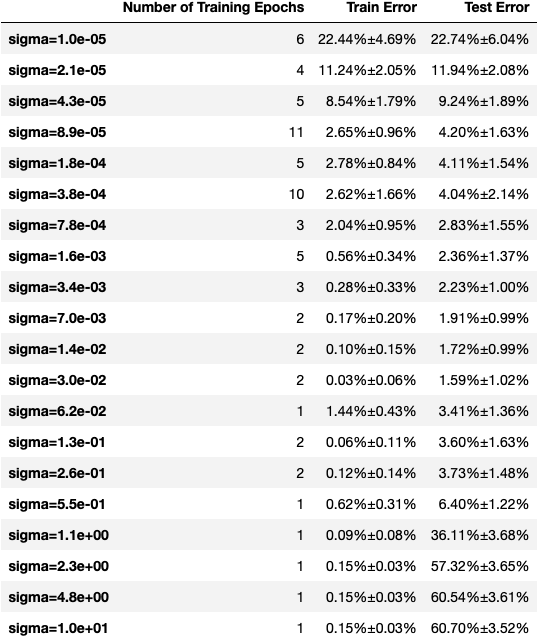
\includegraphics[scale=0.5]{outputs/part1/q5_1-mini.png}
    \caption{Performance for mini data set (to narrow down a hyper-parameter range)}
    \label{fig:7}
    \end{figure}
    \newpage

    Basic Results:

    \begin{figure}[h]
    \centering
    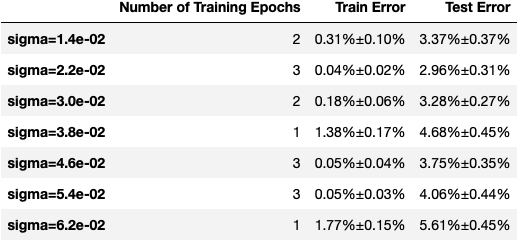
\includegraphics[scale=0.5]{outputs/part1/q5_1.png}
    \caption{20 Runs with a Gaussian Kernel}
    \label{fig:8}
    \end{figure}


    Cross Validation Results:

    \begin{figure}[h]
    \centering
    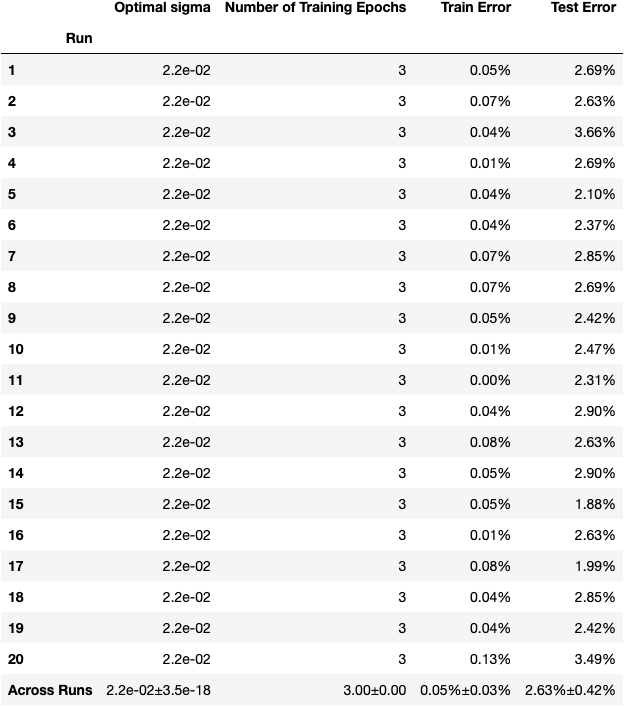
\includegraphics[scale=0.5]{outputs/part1/q5_2.png}
    \caption{5-fold Cross-Validation for 20 Runs with a Gaussian Kernel}
    \label{fig:9}
    \end{figure}

\newpage
    \item[6.] An alternative method to generalise the kernel perceptron to $k$-classes:

    \begin{algorithm}
    \caption{Another training algorithm for multi-class kernel perceptron}\label{alg:cap}
    \begin{algorithmic}
    \For{$k\in\{1, 2, ..., K\}}$ \Comment Initialise weights for first training example
        \State $w^{1, 1}_k \gets 0$
    \EndFor

    \For{$i\in\{1, 2, ..., M\}$}: \Comment Number of Epochs
        \For{$j\in\{2, ..., N\}}$ \Comment Number of training points
            \For{$k\in\{1, 2, ..., K\}}$ \Comment Number of classes
                \State $\hat{y}_k^{i, j} \gets  \sum_{i'=1}^{i-1} \sum_{j'=1}^{j-1} ( w^{i, j}_k \cdot  k(\textbf{x}_{j'}, \textbf{x}_j)} )$ \Comment{Prediction for class $k$ with kernel $k(\cdot, \cdot)$}
            \EndFor
            \State $\hat{c} \gets argmax_k \hat{y}_k^{i, j}$ \Comment Predicted class
            \State $c \gets argmax_k y_k^{i, j}$ \Comment Actual class
            \If{$\hat{c} \neq c$} \Comment Compare predicted and actual class
                \State $w^{i, j}_{c} \gets y_{c}^{i, j}$ \Comment Non-zero weights only for actual and predicted classes
                \State $w^{i, j}_{\hat{c}} \gets y_{\hat{c}}^{i, j}$
                \State $w^{i, j}_{k} \gets 0 \forall k\in\{1, 2, ..., K\}, k \neq c, k\neq \hat{c}$
            \Else \Comment All zero weights if actual and predicted classes match
                \State $w^{i, j}_{k} \gets 0 \forall k\in\{1, 2, ..., K\}$
                \EndIf
        \EndFor
    \EndFor
    \end{algorithmic}
    \end{algorithm}
\newpage

    Basic Results:

    \begin{figure}[h]
    \centering
    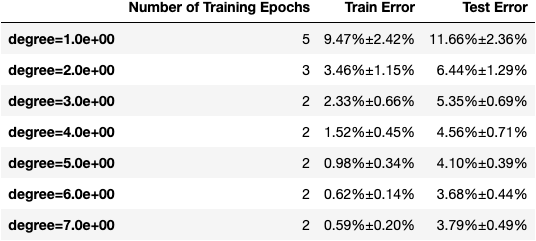
\includegraphics[scale=0.5]{outputs/part1/q6.png}
    \caption{}
    \label{fig:10}
    \end{figure}
    Cross Validation Results:

    \begin{figure}[h]
    \centering
    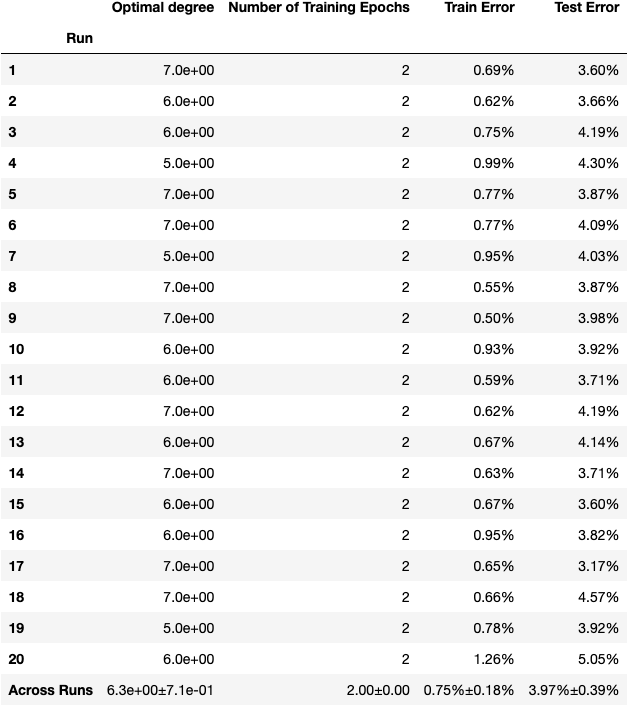
\includegraphics[scale=0.5]{outputs/part1/q6_performance.png}
    \caption{}
    \label{fig:11}
    \end{figure}





\end{itemize}
\newpage
\subsubsection{Discussions}
    Choice of Parameters that weren't cross validated

    Generalisation to k-classifiers

    Kernel Comparison

    Kernel Perceptron Implementation


\newpage
\section{PART II}
\subsection{Semi-supervised Learning via Laplacian Interpolation}

Experimental report for the laplacian interpolation approach:
\\
    \begin{figure}[h]
    \centering
    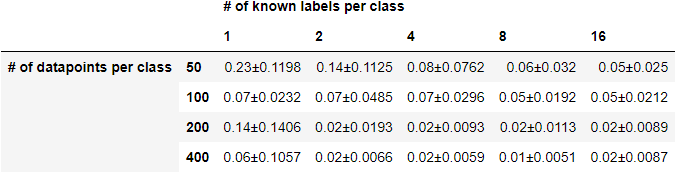
\includegraphics[scale=0.5]{outputs/part2/laplacian_interpolation_report.png}
    \caption{}
    \label{fig:12}
    \end{figure}

\\

And for the laplacian kernel method:
    \begin{figure}[h]
    \centering
    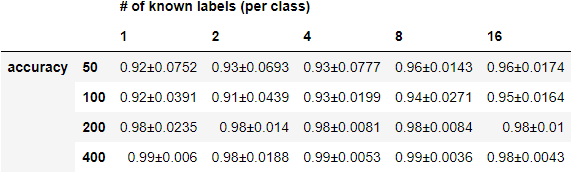
\includegraphics[scale=0.5]{outputs/part2/laplacian_kernel_interpolation_report.png}
    \caption{}
    \label{fig:13}
    \end{figure}

Some observations to make here are:\\


a) Both models seem to perform fairly well, even in the low-data setting.\\

b) Increating the number of known labels increases the accuracy and decreases
 the variance of the predictors.\\

c) Increasing the total number of datapoints generally increases both model accuracies,
and decreases variance. \\

d) The laplacian kernel method outperforms the vanilla inerpolation approach considerably,
on both accuracy and variance. \\


The main reason for the success of this algorithm is the high degree of
 cluster separation observed in the dataset.
\\

For illustration, here is a diagram representing the graph adjacency matrix,
 with colours showing the labelling of an edge. Here blue edges are where both 
labels are -1, teal when both are different, and yellow when both are +1.\\


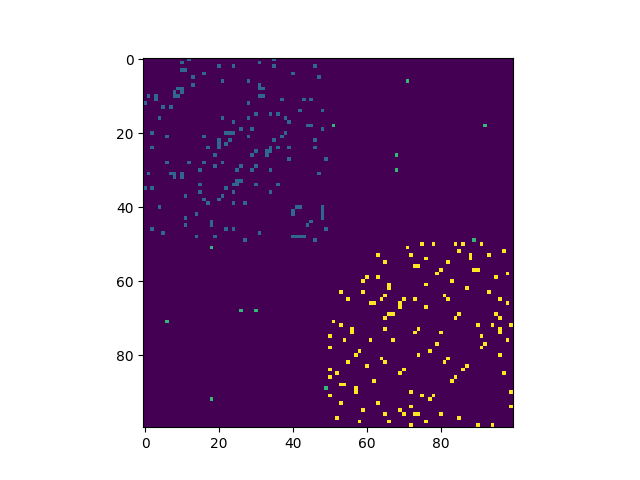
\includegraphics{outputs/part2/graph_label_diagram.png}#

We see through this that the vast majority of datapoints are connected only to points
of the same labelling, and that the graph is highly separated  into 2 clusters.
Hence with minimal training information, both methods are able to predict with a
 high degree of accuracy.\\

Note that error variance decreases as a function of the number of known labels, but 
has a muhc more significant impacgt for the vanilla interpolation method.


We see that the kernel approach consistently outperforms the simple laplacian
 interpolation method. A reasonable explanation for this is that the laplacian
interpolation approach utilises local information to 'diffuse' labels through the graph. 
This means that only datapoints close to labelled data receive information from the 
labels themselves, and accuracy is likely reduced for datapoints far from the labels.
In contrast, the kernel interpolation method takes global information from all the 
labelled datapoints and weights them according to their proximity and connectedness 
to eachother to predict labels.
\newpage



\section{PART III}
\subsection{Questions}
\begin{itemize}
    \item[a.] Sample complexity plots for the four algorithms: perceptron, winnow, least squares, and 1-nearest neighbours.


    \begin{figure}[h]
    \centering
    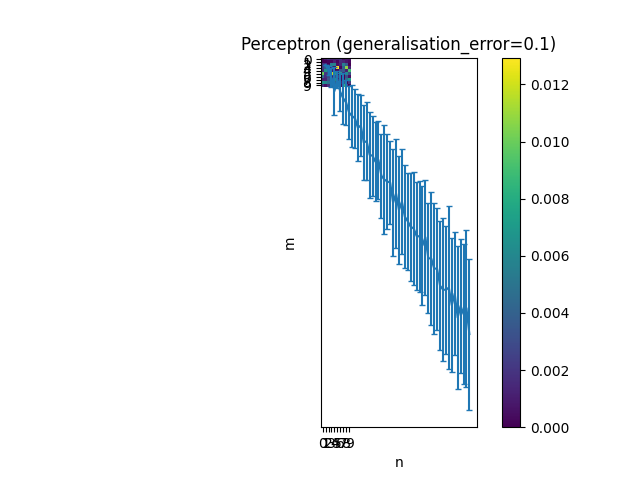
\includegraphics[scale=0.6]{outputs/part3/q1a_perceptron_sample_complexity.png}
    \caption{Perceptron Sample Complexity}
    \label{fig:14}
    \end{figure}


    \begin{figure}[h]
    \centering
    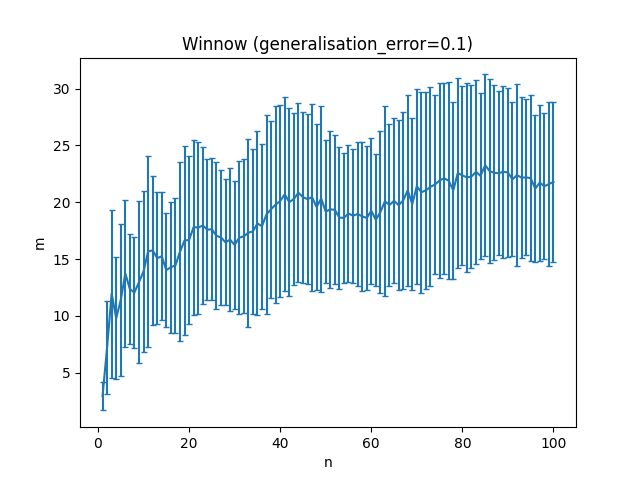
\includegraphics[scale=0.6]{outputs/part3/q1a_winnow_sample_complexity.png}
    \caption{Winnow Sample Complexity}
    \label{fig:15}
    \end{figure}
\newpage
`

    \begin{figure}[h]
    \centering
    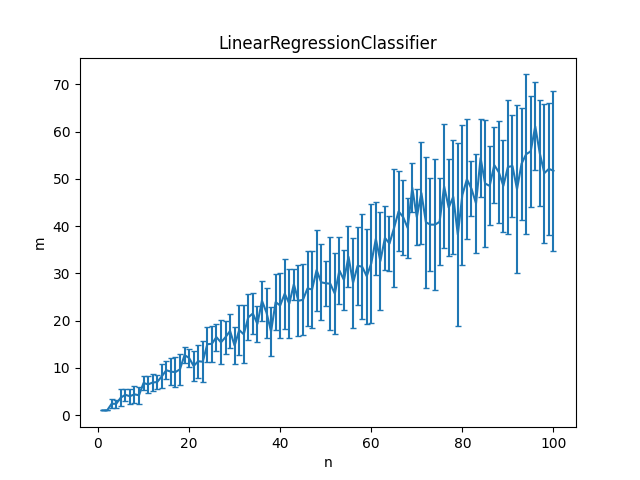
\includegraphics[scale=0.6]{outputs/part3/q1a_lin_reg_sample_complexity.png}
    \caption{Least Squares Sample Complexity}
    \label{fig:16}
    \end{figure}


    \begin{figure}[h]
    \centering
    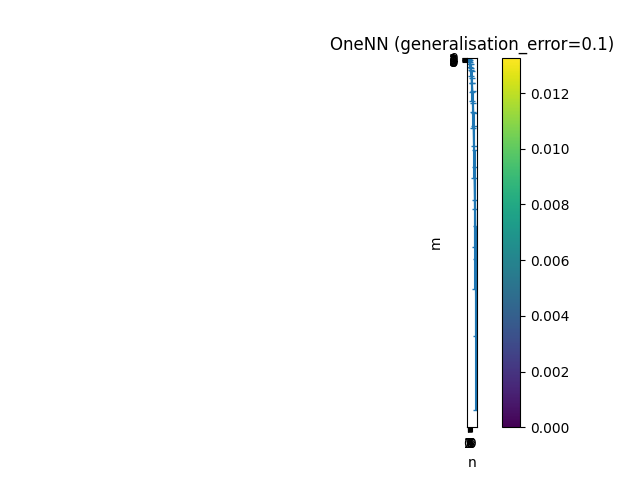
\includegraphics[scale=0.6]{outputs/part3/q1a_one_nn_sample_complexity.png}
    \caption{1-Nearest Neighbours Sample Complexity}
    \label{fig:17}
    \end{figure}


\newpage

    \item[b.] To estimate sample complexity,

    Tradeoffs and biases of this method of sample complexity estimation include
\newpage
    \item[c.] To estimate how $m$ grows as a function of $n$ as $n \rightarrow \infty$ for each of the four algorithms, we first visualise lines of best fit of the sample complexities for different function classes (i.e. polynomial, exponential, logarithm):


    \begin{figure}[h]
    \centering
    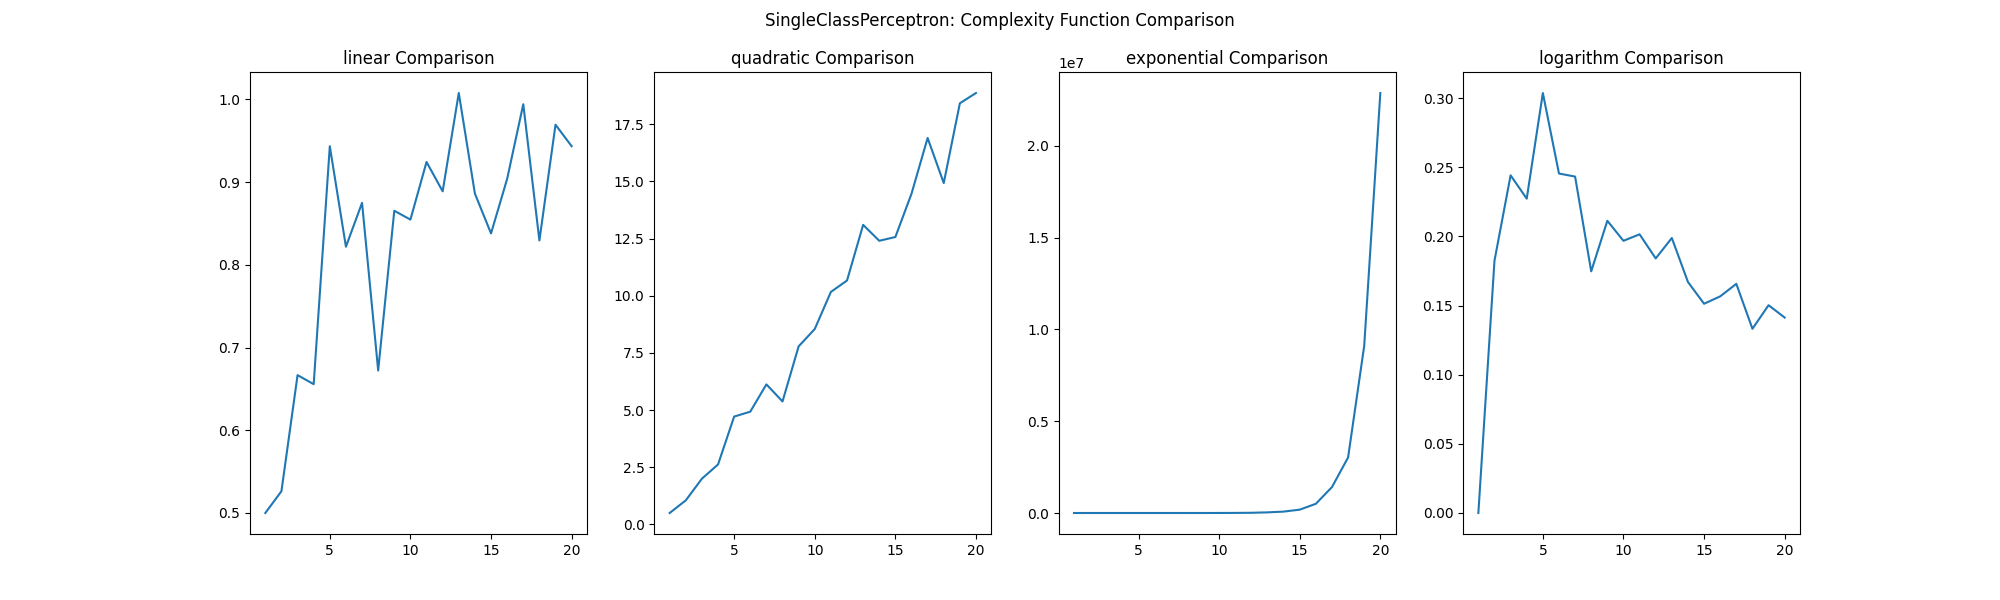
\includegraphics[scale=0.35]{outputs/part3/q1a_perceptron_complexity_function_comparison.png}
    \caption{Perceptron Sample Complexity vs Function Classes}
    \label{fig:18}
    \end{figure}

    \begin{figure}[h]
    \centering
    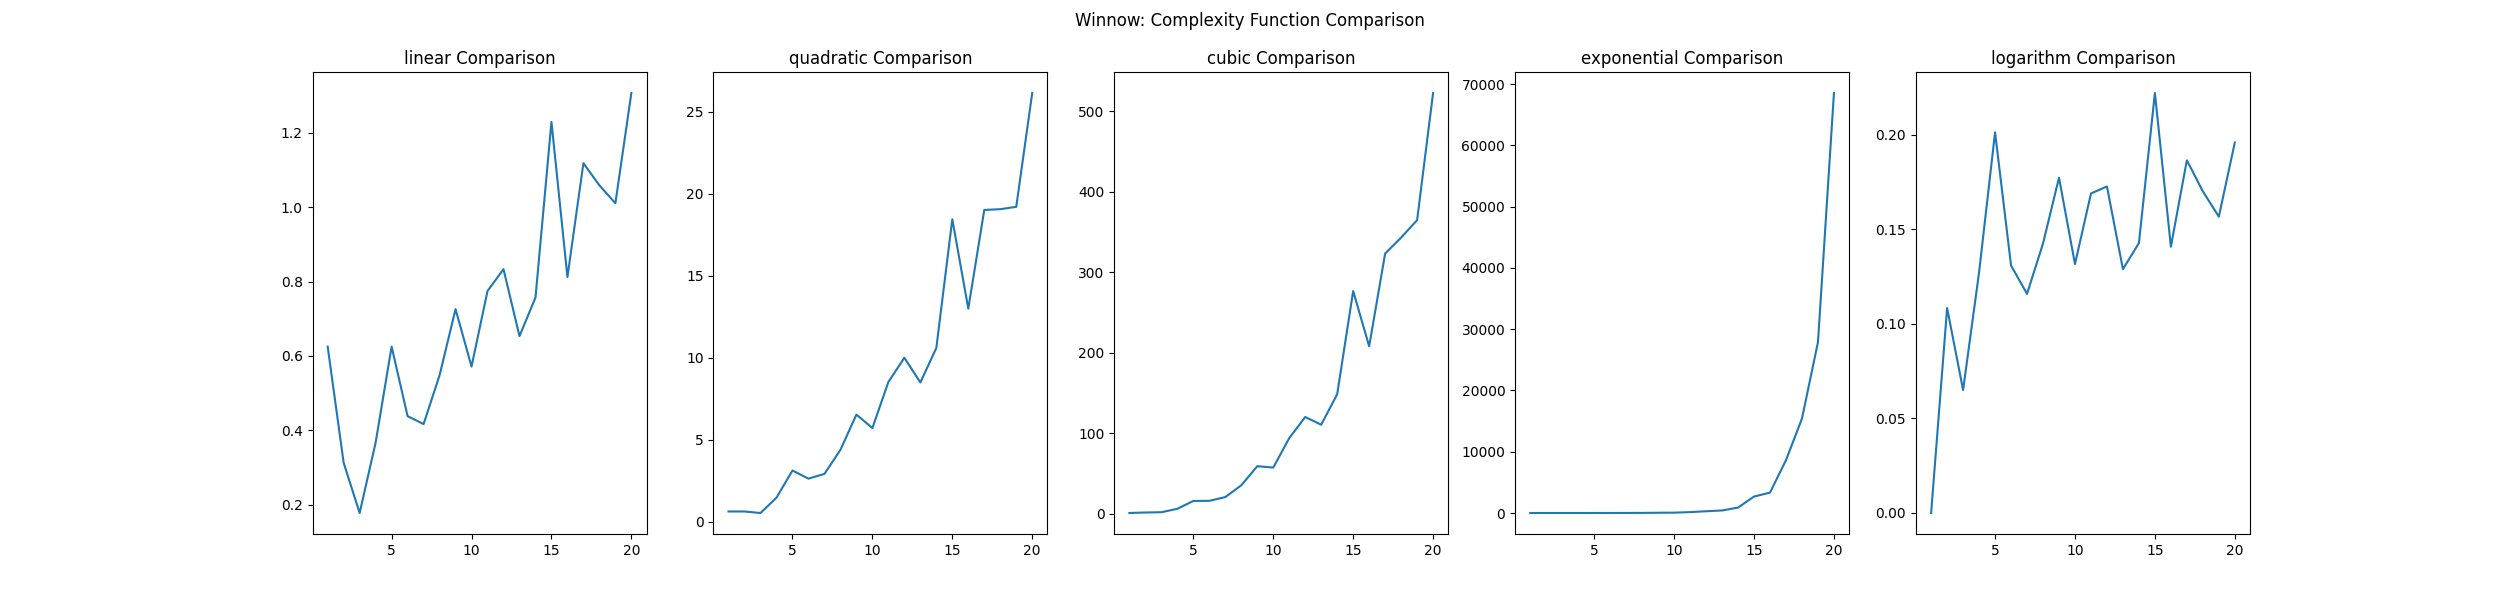
\includegraphics[scale=0.35]{outputs/part3/q1a_winnow_complexity_function_comparison.png}
    \caption{Winnow Sample Complexity vs Function Classes}
    \label{fig:19}
    \end{figure}
\newpage
    \begin{figure}[h]
    \centering
    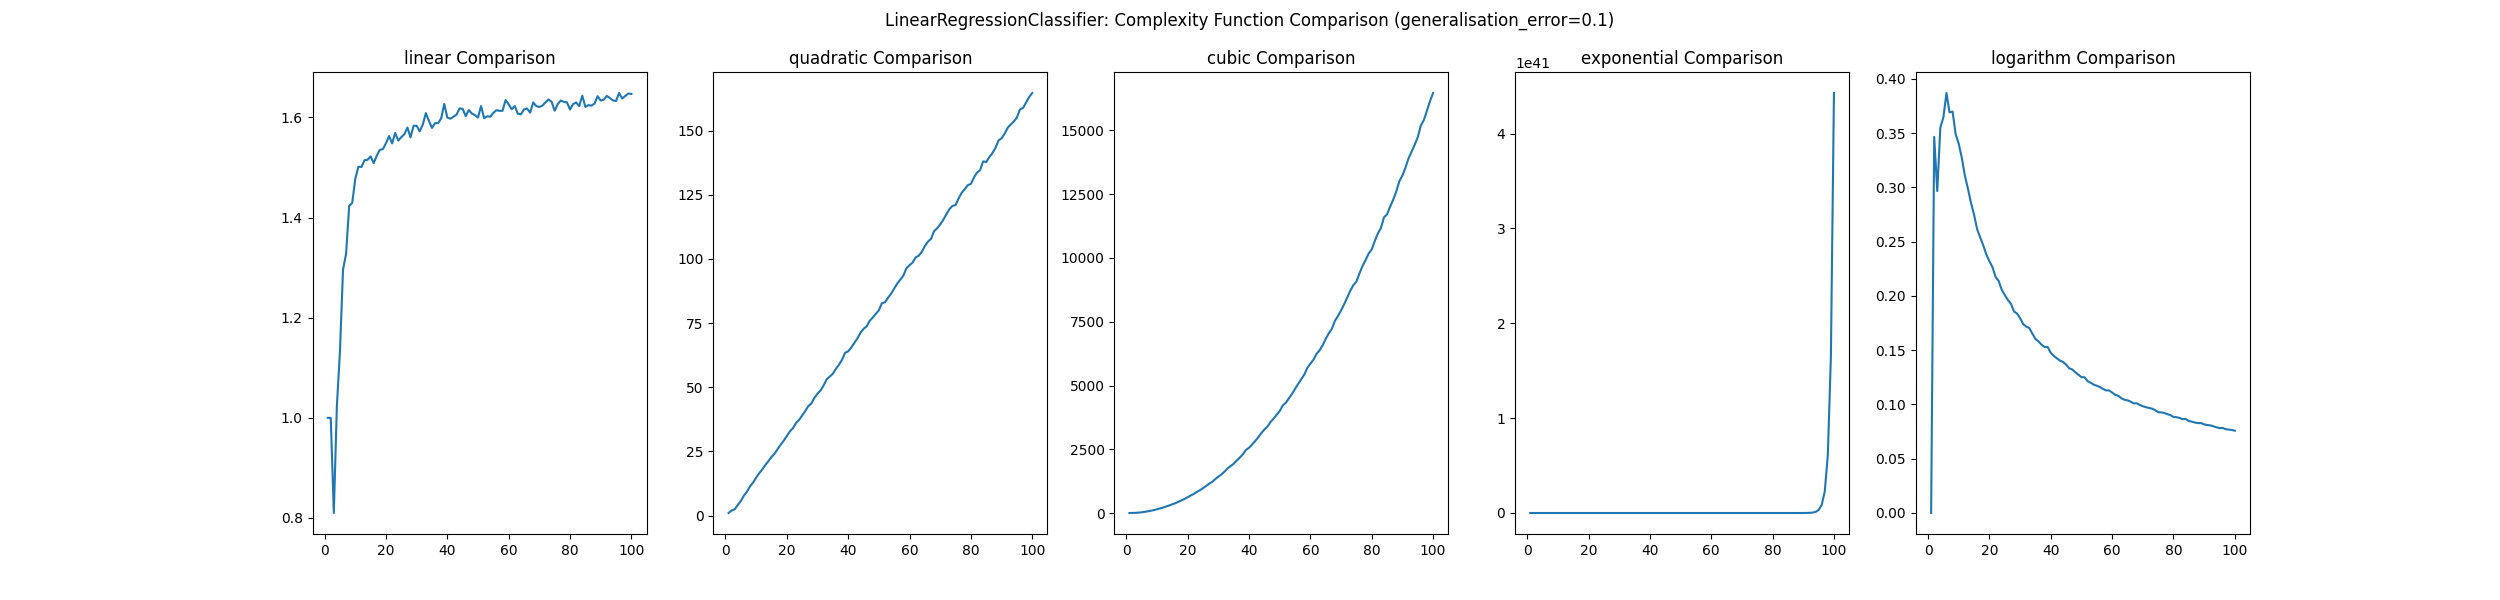
\includegraphics[scale=0.35]{outputs/part3/q1a_lin_reg_complexity_function_comparison.png}
    \caption{Least Squares Sample Complexity vs Function Classes}
    \label{fig:21}
    \end{figure}

    \begin{figure}[h]
    \centering
    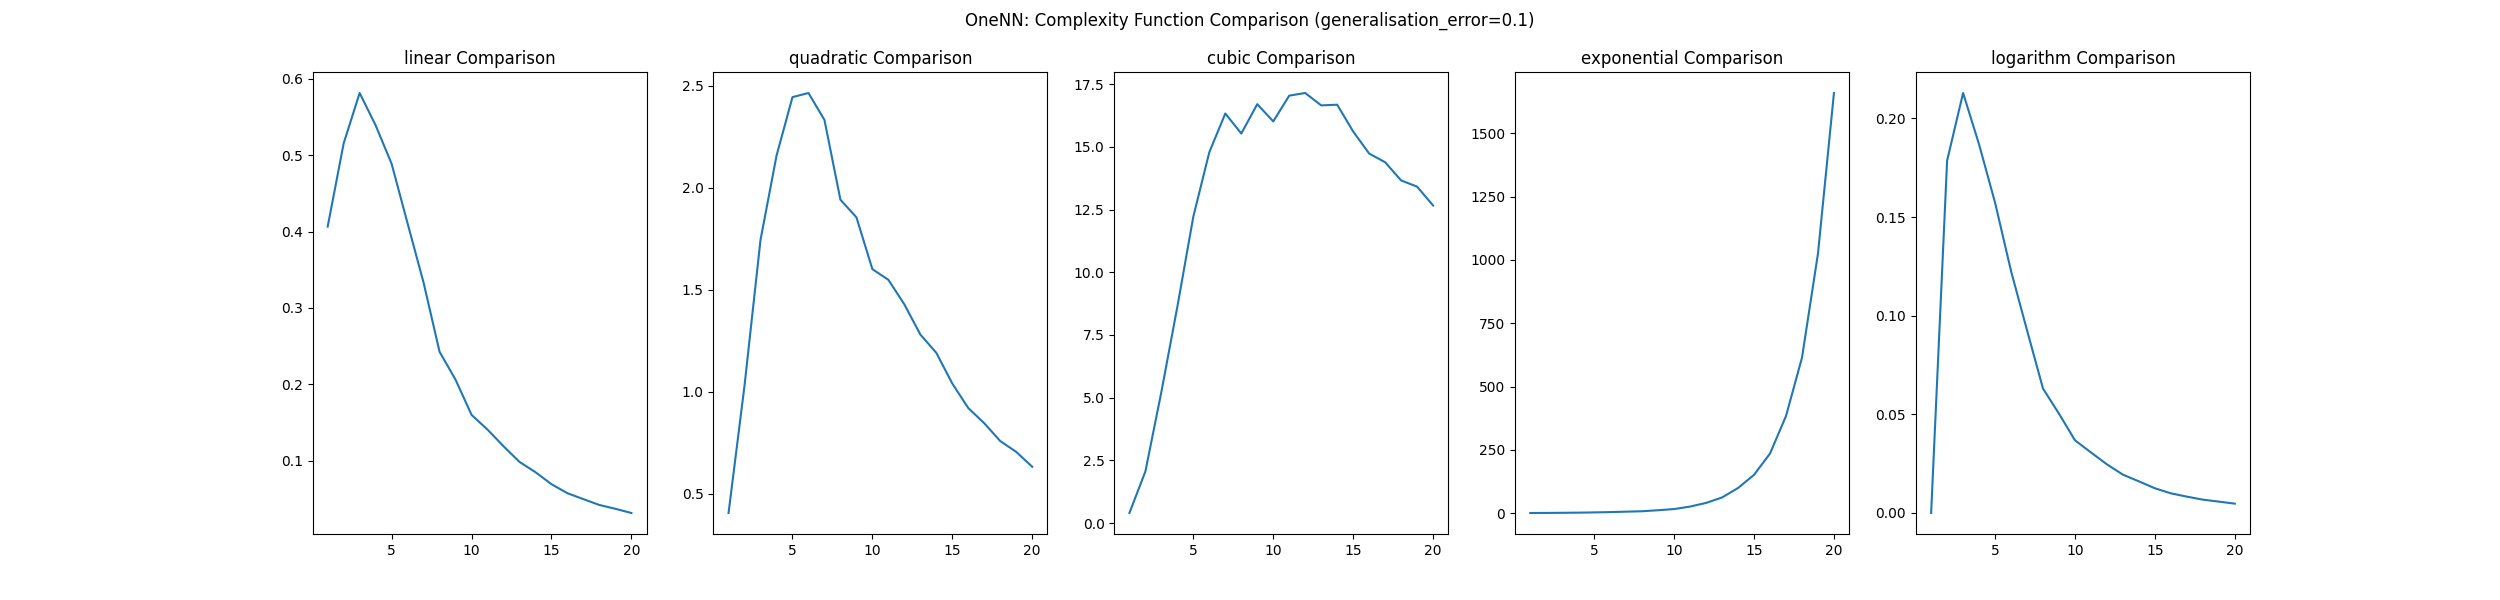
\includegraphics[scale=0.35]{outputs/part3/q1a_one_nn_complexity_function_comparison.png}
    \caption{1-Nearest Neighbours Sample Complexity vs Function Classes}
    \label{fig:22}
    \end{figure}

    From these plots we can see

    Comparing the performance of the four algorithms

\newpage

    \item[d.]\\
    We note that since for any $X_{t}$ , $y_{t} = X_{1,t}$ , we have the following
     expression representing the linear separability of our dataset:\\
    \[(v \cdot x_{t})y_{t} \ge 1\]\\
    Where $v = (1,0, \dots, 0)^{T}$. Note that $\|v\| =1$.\\
    Hence, in our online mistake bound for the perceptron, we have that $\gamma =1$.
    Further note that $\forall t$, $x_{t} \in {-1,1}^{n} \implies \|x_{t}\|^{2}
    = n$. This gives us that $R = max_{t} \|x_{t}\| = \sqrt{n}$.
    Hence our mistake bound for the perceptron algorithm is given by:\\
    
    \[M \le n \].\\

    Using the theorem on page 60 of the online learning notes, we arrive at:\\

    \[Prob(\mathcal{A_{S}}(x ^{\prime}) \ne y^{\prime} ) \le \frac{n}{m}\]\\

\newpage

     \item[e.]\\
     From our experimental observations we may expect the sample complexity of 1-NN
     to be lower bounded by some exponential function. We formalise this in the
     following proposition:\\

    \textbf{Proposition:}\\

    Following the data-generating distribution described above, we have that our sample complexity given by:\\

    $m(n) = \Omega (n)$ \\
    \textbf{Proof:}\\

    Suppose we sample a training set $S = \{(x_{1},y_{1}), \dots, (x_{n},y_{n})\} $ uniformly from the set $\{-1,1\}^{n}$, with associated labels
    defined by the rule $y | x = x_{1}$, and use this training set for inference on an
     arbitrary test point $(x,x_{1})$, sampled uniformly from the same set.
    \\
    We note the following observation:\\

    \textbf{Obs:}\\
    if $x \in S$, then $\mathcal{A}_{S}(x)) = y$, where y is the true label for x. \\

    To justify this, observe that our dataset represents a realiseable learning problem,
    and as such, if $(x,y), (x \prime,y \prime)$ are datapoints sampled from our distribution,
    $x = x \prime \implies y = y \prime $. Trivially, x is the 1-nearest neighbour to itself,
    so the algorithm makes a correct prediction for any datapoint present in our training set.\\

    Hence, $\mathcal{A}_{S}$ makes an error on x $\implies x \notin S$.
    
    Hence, the set of all training sets that make an error on x is contained in the set of all
    training sets not containing x. \\

    Hence, for a given x, $P_{S}(\mathcal{A}_{S}(x) \ne y) \le P_{S}(x \notin S)$.\\

    Since S is a collection of points sampled iid from our data generating distribution, \\
    $P_{S}(x \notin S) = \prod_{i=1}^{m}P(x_{i} \ne x) = \prod_{i}(1 - P(x_{i} = x)) = (1 - 2^{-n})^{m}$\\

    We note that our choice of x was arbitrary, and since we sampled x uniformly, we arrive at the 
    following generalisation error bound:\\

    $\mathbb{E}_{S \sim \mathcal{D}^{m}, x \sim \mathcal{D}}[\mathcal{L}_{S}(x)] \le (1 - 2^{-n})^{m} $\\
    Using the identity $1-x \le e^{-x}$ provided frequently in the notes, we simplify this bound to give:
    \\
    \\

    $\mathbb{E}_{S \sim \mathcal{D}^{m}, x \sim \mathcal{D}}[\mathcal{L}_{S}(x)] \le exp(-2^{n}m)$
    \\
    Suppose we seek m such that our generalisation error is less than some fixed $\epsilon$. \\
    \\
    Hence we require $\mathbb{E}_{S \sim \mathcal{D}^{m}, x \sim \mathcal{D}}[\mathcal{L}_{S}(x)] \le exp(-2^{n}m) \le \epsilon$\\
    \\
    $\implies -m2^{-n} \le log(\epsilon)$\\

    Hence, $m \ge -log(\epsilon)2^{n} = log(\frac{1}{\epsilon}) 2^{n}$\\

    $\implies m = \Omega(2^{n})$\\
    $\square$
\end{itemize}
\end{document}
